\documentclass[12pt, a4paper]{article}
\usepackage{bm, float,amsmath,graphicx,amssymb}
\graphicspath{ {./images/} }
\usepackage[T1]{fontenc}
\usepackage[utf8]{inputenc}
\usepackage{cite}
\usepackage{amsthm}

\title{Overview of the knowledge on minimum graph motion planning problem}
\author{Stepan Yurtsiv, 246437}

\theoremstyle{definition}
\newtheorem{definition}{Definition}[section]

\begin{document}
\maketitle

\section*{Problem description}

We are given a connected, undirected graph $G$ with $n$ vertices. One of the vertices $s$ contains a mobile $robot$.
Each of several other other vertices contains a single moveable $obstacle$. The robot and the obstacles may only reside at vertices, although they may be moved across edges.
A vertex can only contain a single object at a given time (robot/obstacle).
In one step, we may either move the robot or one of the obstacles from its current position $v$ to an adjacent vertex that is not occupied by the robot or an obstacle (in other words a $hole$).
Our goal is to move the robot to a target position $t$ using the smallest number of steps possible.  Let us call this graph motion planning with one robot, or GMP1R for short.

The problem is a simple abstraction of a robot motion planning problem with the geometry replaced by the adjacencies in the graph.
It was first formulated on Proceedings of the 35th Annual Symposium on Foundations of Computer Science (1994) in an article called Motion Planning on a Graph \cite{365740}.

To get an appreciation of how hard the problem is, let us consider a relatively simple instance presented in figure \ref{problem_instance}.

\begin{figure}[H]
  \begin{center}
  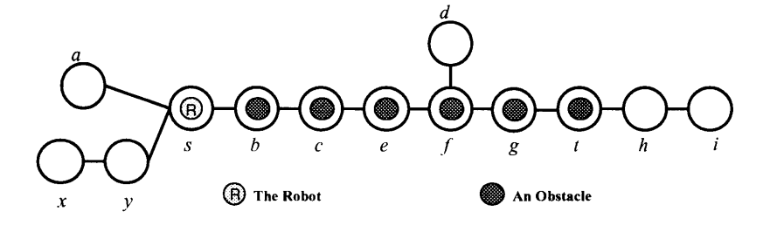
\includegraphics[scale=0.5]{Problem_instance}
  \caption{An instance of GMP1R problem \cite{365740}}
  \label{problem_instance}
  \end{center}
\end{figure}

\noindent
The only feasible plan for moving the robot from $s$ to $t$ is the following:

\begin{enumerate}
    \item Move the robot to $a$
    \item Move the obstacles from $b$ and $c$ to $x$ and $y$
    \item Move all obstacles on a path from $e$ to $t$ two steps to the right
    \item Move the robot to $d$
    \item Move obstacles on $g$ and $t$ to the right past $f$, clearing the way for the robot from $d$ to $t$
\end{enumerate}

As you can see, the path of the robot (and obstacles) may be non-monotone which means sometimes it needs to move away from the target $t$.

\section*{State of the knowledge}

By reduction from 3-SAT authors of the problem \cite{365740} have proven that given an instance of GMP1R and a positive integer $k$, it’s NP-complete to decide whether a solution of length $k$ exists.
The problem remains NP-complete when restricted to a planar graph.

\subsection*{Trees}

If $G$ is a tree, there’s a polynomial time algorithm that computes an optimal plan.
The algorithm itself is quite complex and depends on a lot of definitions, but in the end it boils down to solving $O(n^6)$ mincost flow problems on networks with $O(n)$ nodes each, and a shortest path problem on a graph with $O(n^3)$ nodes (you can read an exact algorithm in \cite{365740} section 2.2). The running time of the algorithm is quite large so the authors of
the problem also presented a faster approximation algorithm that achieves a plan of length at most 7 times the optimal length.
The algorithm is a simplified version of the previous one that requires solving mincost flow problems on at most $n$ networks with
$O(n)$ nodes each.

\subsection*{General graphs}

\begin{definition}[]
We call a path of $G$ a $degree-2$ $chain$ or simply a $chain$
if all of its internal vertices are of degree 2 and neither
of the endpoints is of degree 2.
\end{definition}

No exact polynomial algorithms have been found for GMP1R on general graphs so we need to resort to approximation ones.
A natural heuristic for an approximate solution is to let the robot flow the shortest path from $s$ to $t$, with possible side-stepping.
The plan obtained by this heuristic can be as bad as $\Omega(l_{max})$ times optimal, where $l_{max}$ is the length
of the longest chain in $G$.
It's because a chain of length $l$ packed with obstacles requires
$\Omega(l^2)$ steps to clear, while the optimal plan may choose a slightly longer path with few obstacles.
Another case in which the shortest path performs poorly is when there is a rich pool of holes “closer” to the longer path than the shorter path.
After some in-depth analysis, authors of the problem \cite{365740} present a polynomial time $O(\sqrt n)$-approximation algorithm
for GMP1R on general graphs (\cite{365740} section 3).

\subsection*{Cartesian product graphs}

\begin{definition}[]
  The Cartesian product $G_1 \square G_2$ of two graph $G_1$ and $G_2$ (figure \ref{cartesian}) is a graph with vertex set $V(G_1) \times V(G_2)$ in which
  $(u_i, v_j)$ and $(u_p, v_q)$ are adjacent if one of the
  following conditions holds:

  \begin{enumerate}
    \item $v_j = v_q$ and ${u_i,u_p} \in E(G_1)$
    \item $u_i = u_p$ and ${v_j,v_q} \in E(G_2)$
  \end{enumerate}
\end{definition}

\begin{figure}[H]
  \begin{center}
  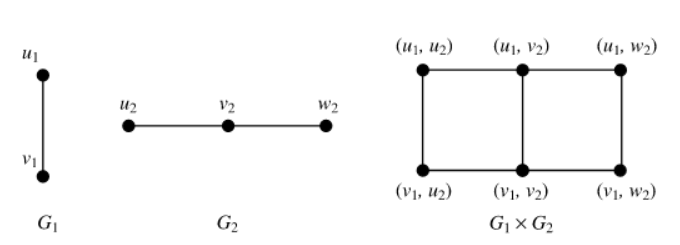
\includegraphics[scale=0.5]{Cartesian.png}
  \caption{Cartesian product of two graphs}
  \label{cartesian}
  \end{center}
\end{figure}

Consider a version of GMP1R with $n-2$ obstacles, i.e. there’s
a single hole. The authors of \cite{deb2014motion} showed that the
path traced by the robot coincides with a shortest path in case of Cartesian product graphs.
They also gave the minimum number of moves required for the motion planning problem in the Cartesian product of two graphs having 
girth (length of the shortest cycle in a graph) 6 or more,
but it requires too much definitions to fully express it in this overview.

\subsection*{Lexicographic product graphs}

\begin{definition}[]
  The Cartesian product $G_1 \circ G_2$ of two graph $G_1$ and $G_2$ (figure \ref{lexic}) is a graph with vertex set $V(G_1) \times V(G_2)$ in which
  $(u_i, v_j)$ and $(u_p, v_q)$ are adjacent if one of the
  following conditions holds:

  \begin{enumerate}
    \item ${u_i,u_p} \in E(G_1)$
    \item $u_i = u_p$ and ${v_j,v_q} \in E(G_2)$
  \end{enumerate}
  Unlike Cartesian product, the lexicographic product is not commutative,
  i.e. $G_1 \circ G_2$ is not the same as $G_2 \circ G_1$.
\end{definition}

\begin{figure}[H]
  \begin{center}
  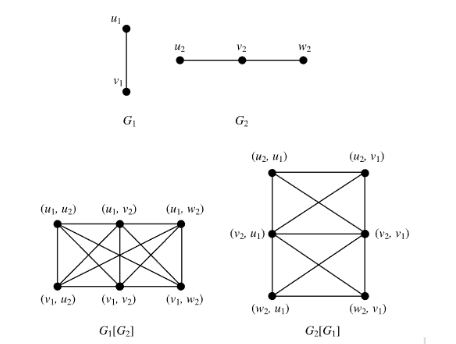
\includegraphics[scale=0.7]{Lexic.png}
  \caption{Lexicographic product of two graphs}
  \label{lexic}
  \end{center}
\end{figure}

Akwu and Oyewumi in \cite{akwu2018motion} showed the minimum number of moves required for the motion planning problem in lexicographic products of some graphs.
In addition, they proved the necessary and sufficient condition
for the connectivity of the lexicographic product of two graphs.

\section*{Similar problems}

A generalisation of GMP1R is GMP$k$R, where there are $k$ robots with respective destinations. A special case of GMP$k$R, in which there are no obstacles, has been studied previously. Wilson \cite{wilson1974graph} studies the case $k=n-1$  and gives an efficiently checkable characterization of the solvable instances of the problem. 
Kornhauser, Miller, and Spirakis \cite{kornhauser1984coordinating}
extend his result to any $k \leq n-1$ and also give an upper
bound of $O(n^3)$ on the number of steps to solve any solvable instance. They give an example showing that this bound is the best possible. 
Goldreich \cite{goldreich1984shortest} has studied the complexity of determining the shortest move sequence for the GMP$k$R problem
and shown that this is NP-hard in the case $k=n-1$.

\bibliographystyle{plain}
\bibliography{References}

\end{document}

